\documentclass[border=14pt]{standalone}
\usepackage[T1]{fontenc}
\usepackage[default]{sourcesanspro}
\usepackage{tikz}
\usetikzlibrary{arrows.meta}

% Blank coordinate system for the Fahrrad / MSE exercise
%   x-axis: Strecke in km (0..10),  scale x=0.8cm per unit
%   y-axis: Zeit in Minuten (0..50), scale y=0.12cm per unit
%   Grid: vertical every 1 km, horizontal every 5 min

\begin{document}
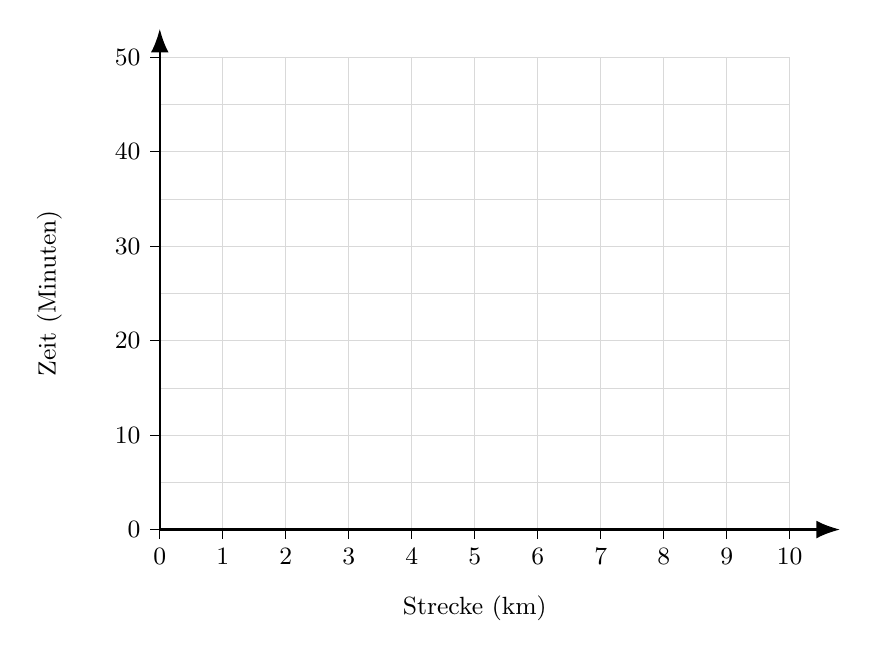
\begin{tikzpicture}[x=0.8cm, y=0.12cm]

  % --- Grid ---
  \foreach \x in {0,...,10} \draw[gray!30, very thin] (\x, 0) -- (\x, 50);
  \foreach \y in {0,5,...,50} \draw[gray!30, very thin] (0, \y) -- (10, \y);

  % --- Axes ---
  \draw[thick,-{Latex[length=3mm]}] (0,0) -- (10.8,0);
  \draw[thick,-{Latex[length=3mm]}] (0,0) -- (0,53);

  % --- X ticks ---
  \foreach \x in {0,...,10} {
    \draw (\x, 0) -- (\x, -1) node[below, font=\small] {\x};
  }
  \node[font=\small, anchor=north] at (5, -6) {Strecke (km)};

  % --- Y ticks ---
  \foreach \y in {0,10,20,30,40,50} {
    \draw (0, \y) -- (-0.15, \y) node[left, font=\small] {\y};
  }
  \node[font=\small, rotate=90, anchor=south] at (-1.4, 25) {Zeit (Minuten)};

\end{tikzpicture}
\end{document}
